Creamos  la función \texttt{TaskBatch} en el archivo \texttt{task.cpp}. Nuevamente la implementación es muy sencilla.

Tenemos una variable \texttt{tiempo\_disponible}, que guarda el tiempo disponible de la tarea para ser usado en el CPU sin contar el tiempo que se necesita para lanzar las llamadas bloqueantes (el cual es de un ciclo por llamada).

Si los parámetros son coherentes, es decir que no se pide hacer más llamadas bloqueantes de las que es posible con el tiempo dado, entonces se itera sobre la cantidad de bloqueos, pasado por parámetro. En cada iteración se decide, de forma pseudo-aleatoria, cuánto del tiempo disponible del CPU se va a utilizar antes de hacer el respectivo bloqueo. Una vez usado el CPU por dicha cantidad de tiempo, se procede a actualizar \texttt{tiempo\_disponible} y se lanza el pedido de \emph{I/O}.

Una vez que se realizaron todos los bloqueos, se gasta en el CPU el tiempo disponible que pudiera haber sobrado (de no haberlo simplemente se prosigue con la finalización del proceso).

La figura \ref{fig:ej3} ilustra un lote de 4 tareas de este tipo.
%%%No se me ocurre que podría rescatarse de esto%%%

\begin{figure}[H]
  \centering
  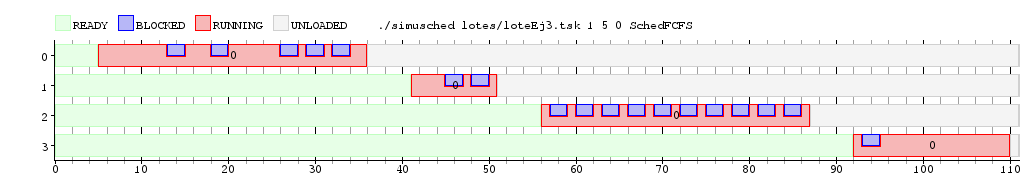
\includegraphics[width=1\textwidth]{img/imgEj3}
  \caption{}
  \label{fig:ej3}
\end{figure}